\part{Monitoring and Autoscaling}

\section{Cloud Monitoring}

\subsection{Introduction \& Definitions}
\begin{itemize}
	\item Motivation: get data about the running system to make \textbf{best use of resources} at \textbf{lowest cost}.
	\begin{itemize}
		\item cloud infrastructure: resource management, root cause analysis, accounting \& metering, incident detection
		\item cloud applications: performance analysis, resource management, failure detection and debugging, SLA verification
	\end{itemize}
	\item Definition:
	\paragraph{Monitoring} the process of \textbf{collecting status information} of applications and resources to observe application and infrastructure.
	\paragraph{Monitoring System} components for gathering monitoring data at runtime -- \textbf{the target system(HW/SW), raw data and data storage}.
	\begin{itemize}
		\item requirements: comprehensive, low intrusion, extensibility, scalability, elasticity, accuracy, resilience
		
	\end{itemize}
	\paragraph{Target System} system to be monitored. an \textbf{online system}
	\begin{itemize}
		\item status depends not only on the \textbf{codes} but also the \textbf{environment} where it runs(\#VMs running on physical machines, bandwidth, cloud storage)
		
		$\rightarrow$ execution is \textbf{not reproducible}
		\item \textbf{real-time analysis} and \textbf{continuous data collection}
	\end{itemize}
	
	\paragraph{Analysis Tools} tools that read monitoring data from data storage.
	\paragraph{Informations}
	\begin{itemize}
		\item Alerts: alarm of exceeding thresholds. eg: CPU utilization 100\%, full storage
		\item Dashboard: overview of resources
		\item Costs: billing and usage of resources
		\item Bottleneck: most critical service/program that slows down response time/ most CPU time
		\item Root cause: once bottleneck defined, find out the root cause
		\item etc.
	\end{itemize}

	\paragraph{Blackbox Monitoring} \textbf{no data} are gained from \textbf{inside} of the monitored system(blackbox). A request interface, no visibility of internal system structure. eg: state of service like CPU/disk usage
	
	\paragraph{Whitebox Monitoring} data \textbf{also gained} from \textbf{inside} of the monitored system. eg: metrics specific to application \#requests
\end{itemize}

%\subsection{Metrics for Monitoring} \label{metrics}
%\begin{itemize}
%	\item Typical metrics:
%	\begin{itemize}
%		\item \textbf{latency}: response time
%		\item \textbf{throughput}: \#requests/sec, network I/O rate, concurrent sessions, \#transactions/sec 
%		\item \textbf{error rate}: rate of fail requests. 
%		\item utilization: CPU time/percentage, memory percentage, disk queue length(I/O)
%	\end{itemize}
%	
%	\item monitoring in different cloud layers:
%	\begin{figure}[H]
%		\centering
%		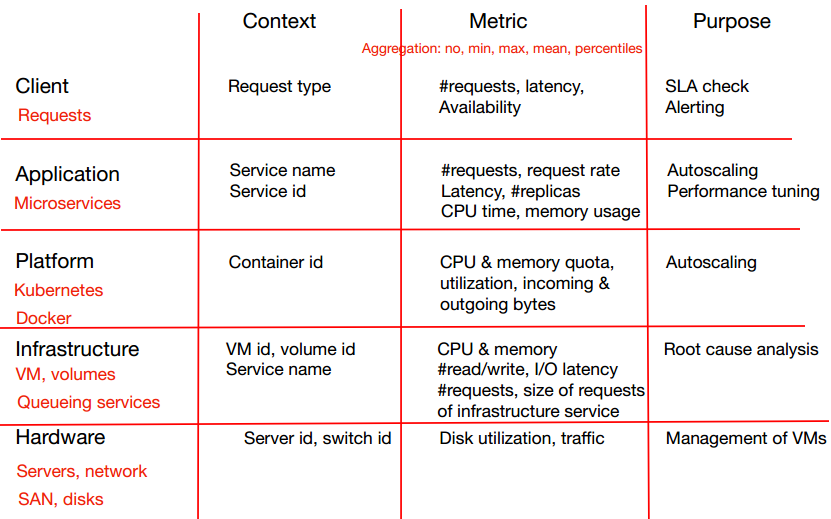
\includegraphics[width=\textwidth]{monitoring.png}
%	\end{figure}
%\end{itemize}



\subsection{Three Pillars/ Data Sources of Monitoring: Logs, Metrics, Traces}

\subsubsection{Logs}
\begin{itemize}
	\item Definition: a sequence of immutable records of discrete events.
	\item Characteristics:
	\begin{itemize}
		\item forms: plain texts, structured (eg: JSON), binary
		\item high level of detail, different levels possible
		\item hard to read and analyze
	\end{itemize}
	\item Techniques of Processing and Analyzing Logs: \textbf{ELK Stack}
	\begin{itemize}
		\item Beats \& Logstash: data ingestion. read, process logs and insert into Elastic Search.
		\item Elastic Search: search, analyze and store data
		\item Kibana: data visualization
	\end{itemize}
	\item Other providers: AWS CloudWatch Log Insights
	
\end{itemize}

\subsubsection{Metrics}
\begin{itemize}
	\item Typical metrics:
	\begin{itemize}
		\item \textbf{latency}: response time
		\item \textbf{throughput}: \#requests/sec, network I/O rate, concurrent sessions, \#transactions/sec 
		\item \textbf{error rate}: rate of fail requests. 
		\item utilization: CPU time/percentage, memory percentage, disk queue length(I/O)
	\end{itemize}
	
	\item monitoring in different cloud layers:
	\begin{figure}[H]
		\centering
		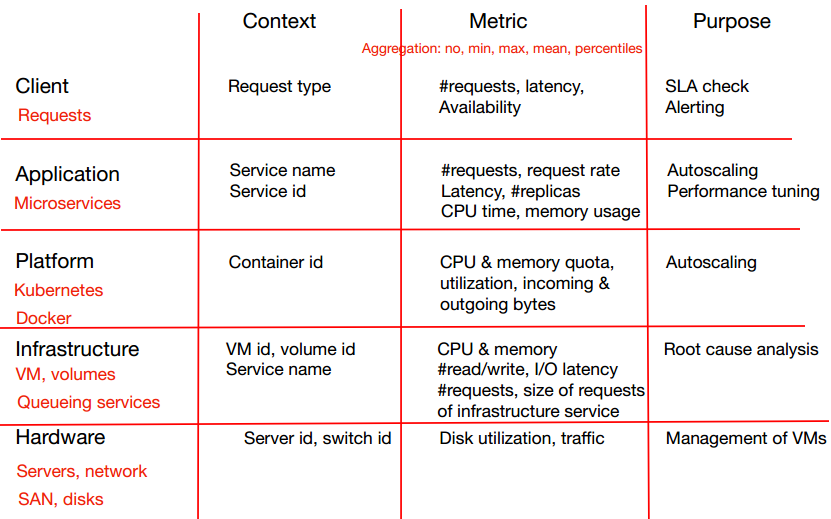
\includegraphics[width=\textwidth]{monitoring.png}
	\end{figure}
	\item Techniques for Processing and Analyzing Metrics: \textbf{Prometheus} (open source)
	\begin{itemize}
		\item data collection, storage \& querying: \textbf{time series} data
		\item Architecture:
		\begin{itemize}
			\item \textbf{server}: retrieved metrics saved in TSDB/storage, HTTP-server for data querying and analysis
			\item \textbf{target discovery}: define monitored targets 
			\item \textbf{metric retrival}: scraping at endpoint /metrics from target, pull for long-lived jobs, push gateway for short-lived jobs
			\item \textbf{alert manager}: receives alerts from server and send to various channels
			\item \textbf{data visualization}: Grafana
			
		\end{itemize}
		\item Scalability: \textbf{hierarchical}. Global DC stores aggregated data, local DC stores more detailed data.
		\begin{figure}[H]
			\centering
			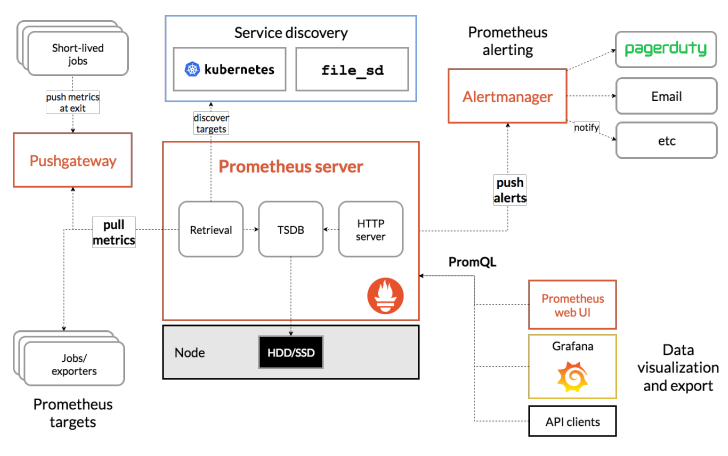
\includegraphics[width=0.8\textwidth]{prometheus.png}
		\end{figure}
		\item Other providers: AWS CloudWatch (custom and user-defined metrics)
	\end{itemize}
\end{itemize}

\subsubsection{Traces}
\begin{itemize}
	\item Definition: Finding out \textbf{interaction} of different services/events and \textbf{association of sequence}.
	\item Techniques for Processing and Analyzing Traces: \textbf{Google Dagger}
	\begin{itemize}
		\item \textbf{global request ID}: each event has a \textbf{trace ID} created at front-end service. It's \textbf{passed down} to subrequests.
		\item representation: \textbf{Dapper trace tree}
		\begin{itemize}
			\item nodes: \textbf{spans}, lifetime of a request. It has a \textbf{trace ID, parent ID and span ID}.
			\item edges: temporal relationship of calls
		\end{itemize}
		\item trace collection: logs --> dapper collectors --> into central bigtable(trace IDs and span IDs)
%	    \begin{itemize}
%	    	\item \textbf{span data} is written in local \textbf{log files}.
%	    	\item \textbf{dapper collector} reads files from all production hosts 
%	    	\item  \textbf{trace IDs and span IDs} are written to a cell in a \textbf{sparse Dapper Bigtable}
%	    \end{itemize}
	
	
		\item possible challenges: 
		\begin{itemize}
			\item clock skew from different servers in distributed system.
			\item \textbf{overheads}: caused by the massive amount of requests, trace generation and collection. Reduction by coalescing, adaptive sampling(application/trace id), asynchronous writes 
		\end{itemize}
		
		
	\end{itemize}
\end{itemize}




















\subsection{Challenges in Monitoring: Overheads}
\begin{itemize}
	\item Definition: overhead is any \textbf{combination of excess or indirect computation time, memory, bandwidth, or other resources} that are required to perform a specific task.  Such resource \textbf{doesn't contribute directly} to the result, but it's \textbf{required} to make it work.
	
	\item Reasons: 
	\begin{itemize}
		\item collection of data: \textbf{all available}
		\item instrumentation: insert additional binary calls/codes in the program and use these calls to trace native calls and achieve measurement goals
		\item aggregation computation
		\item memory overhead for buffering
		\item storage overhead for long-term storage
	\end{itemize}
	
	
	
	\item Reduction techniques: 
	\begin{itemize}
		\item reduce \textbf{number} of metrics: collect only important metrics
		\item reduce measurement \textbf{frequency}
		\item representation: choose \textbf{binary} instead of ASCII
		\item message \textbf{coalescing}: package multiple messages into one message
		\item \textbf{sampling}
		\item long-term \textbf{coarsening}: after some time period, only store \textbf{aggregated} values
	\end{itemize}
\end{itemize}




